\section{Dataset Analysis}
\label{sec:dataset-analysis}

To assess whether Open-AoE exhibits a distinctive data profile beyond dataset scale, we compare it with OpenEgo~\cite{openegocentric2025}, EgoDex~\cite{egodex2025}, and EgoXtreme~\cite{egoxtreme2026} across four complementary dimensions: visual representation diversity, semantic and temporal supervision, annotation consistency, and downstream training utility. %
Approximately 100 hours of data are included for Open-AoE, OpenEgo, and EgoDex, whereas EgoXtreme is evaluated using its entire available release because its total duration is substantially smaller. %
The analysis therefore focuses not only on the breadth of the visual and semantic distributions, but also on the completeness, consistency, and practical usability of the associated supervision.

\begin{figure*}[t]
    \centering
    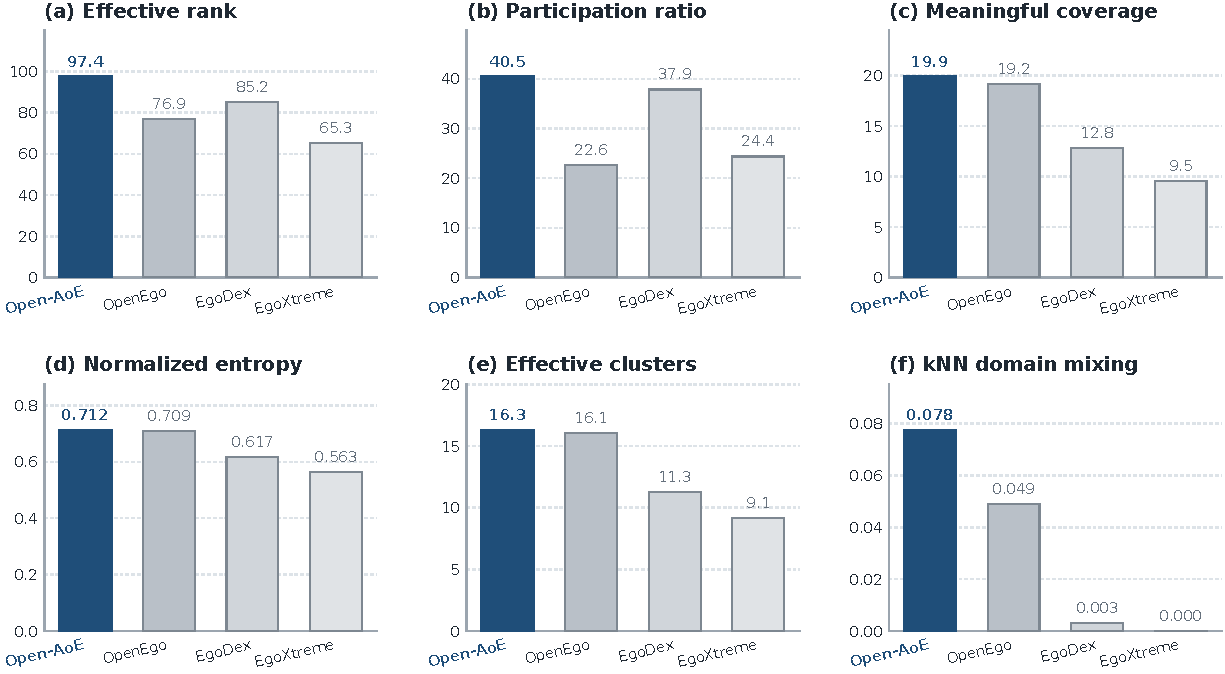
\includegraphics[width=\linewidth]{figures/fig_clip_six_metrics.pdf}
    \caption{High-dimensional CLIP feature analysis. Bars report the mean over 3,000 balanced random subsamples, with 2,000 embeddings drawn from each dataset in every trial. Open-AoE has the highest mean in all six metrics.}
    \label{fig:clip_six_metrics}
\end{figure*}

\subsection{High-Dimensional Visual Diversity}

We use CLIP~\cite{radford2021clip} image embeddings to compare the visual feature distributions of the four datasets. %
Visual frames are sampled from each video sequence and encoded using the CLIP image encoder. %
Each embedding is then $\ell_2$-normalized, yielding $\mathbf{z}_i\in\mathbb{R}^{D}$, where $i$ indexes a sampled visual observation and $D$ is the CLIP feature dimension. %
To control for unequal dataset sizes, we conduct 3,000 balanced random trials, each sampling 2,000 embeddings without replacement from every dataset. %
All reported values are averaged across these trials.

We first examine the covariance spectrum of each dataset in the original normalized CLIP space. %
For dataset $s$, let $\lambda_{s,j}$ denote the $j$-th eigenvalue of its embedding covariance matrix, where $j=1,\ldots,D$, and let $p_{s,j}$ be the corresponding proportion of total variance. %
Effective Rank is the exponential entropy of the normalized covariance spectrum, whereas Participation Ratio measures its inverse concentration:
\begin{equation}
p_{s,j}=\frac{\lambda_{s,j}}{\sum_r\lambda_{s,r}},
\qquad
R_{\mathrm{eff}}^{(s)}
=\exp\!\left(-\sum_j p_{s,j}\log p_{s,j}\right),
\qquad
R_{\mathrm{PR}}^{(s)}
=\frac{\left(\sum_j\lambda_{s,j}\right)^2}
{\sum_j\lambda_{s,j}^{2}}.
\end{equation}
Both metrics estimate the effective number of feature directions that carry substantial variance. %
Higher values therefore indicate that visual variation is distributed across a larger set of active directions rather than being concentrated in a few dominant modes.

We next measure how broadly and evenly each dataset occupies a shared visual feature partition. %
In each trial, the pooled balanced embeddings are transformed using a common PCA representation and partitioned into a shared codebook of $K=50$ cells. %
Let $n_{s,c}$ denote the number of embeddings from dataset $s$ assigned to cell $c$, and let $q_{s,c}$ denote the corresponding occupancy proportion. %
Meaningful Coverage counts cells containing at least $\tau$ samples, while Normalized Cluster Entropy and Effective Clusters quantify the balance of the occupancy distribution:
\begin{equation}
\begin{aligned}
q_{s,c}
&=\frac{n_{s,c}}{\sum_{u=1}^{K}n_{s,u}},
&
C_{s,\tau}
&=\sum_{c=1}^{K}\mathbf{1}\!\left[n_{s,c}\ge\tau\right],
\\
H_{\mathrm{norm}}^{(s)}
&=-\frac{\sum_{c=1}^{K}q_{s,c}\log q_{s,c}}{\log K},
&
N_{\mathrm{eff}}^{(s)}
&=\exp\!\left(-\sum_{c=1}^{K}q_{s,c}\log q_{s,c}\right).
\end{aligned}
\end{equation}
Here, $C_{s,\tau}$ denotes the number of visual regions with sufficiently stable sample support, with $\tau=5$ used throughout our experiments. %
$H_{\mathrm{norm}}^{(s)}$ measures how evenly the samples are distributed across the shared codebook, while $N_{\mathrm{eff}}^{(s)}$ expresses the same entropy as an equivalent number of uniformly occupied cells. %
Higher values indicate broader and more balanced coverage of the shared visual feature space.

Finally, we compute kNN Domain Mixing directly in the original normalized CLIP space, without codebook discretization. %
Let $y_i$ denote the dataset identity of embedding $i$, let $N_s$ be the number of sampled embeddings from dataset $s$, and let $\mathcal{N}_k(i)$ denote the set of its $k$ nearest neighbors in the pooled sample. %
The metric is defined as
\begin{equation}
M_{\mathrm{kNN}}^{(s)}
=
1-\frac{1}{N_s}
\sum_{i:y_i=s}
\frac{1}{k}
\sum_{j\in\mathcal{N}_k(i)}
\mathbf{1}\!\left[y_j=s\right],
\end{equation}
where $\mathbf{1}[\cdot]$ is the indicator function and $k=20$. %
The inner term measures the proportion of same-dataset neighbors around an embedding; therefore, $M_{\mathrm{kNN}}^{(s)}$ is the average proportion of neighboring samples originating from other datasets. %
A higher value indicates stronger local connectivity to a broader range of visual domains.

As shown in Fig.~\ref{fig:clip_six_metrics}, across the 3,000 balanced trials, Open-AoE achieves the highest mean in all six metrics: Effective Rank ($97.43$), Participation Ratio ($40.47$), Meaningful Coverage ($19.89$), Normalized Cluster Entropy ($0.712$), Effective Clusters ($16.29$), and kNN Domain Mixing ($0.0775$). %
The largest advantages are observed in Effective Rank and kNN Domain Mixing, indicating that Open-AoE spans a larger number of active feature directions while maintaining stronger local connectivity to other visual domains. %
Moreover, Open-AoE ranks first in Effective Rank, Participation Ratio, and kNN Domain Mixing in all 3,000 trials. %
Its advantages in the coverage- and entropy-based metrics are smaller, particularly relative to OpenEgo, but their repeated-sampling means remain the highest among all four datasets.

\begin{figure*}[t]
    \centering
    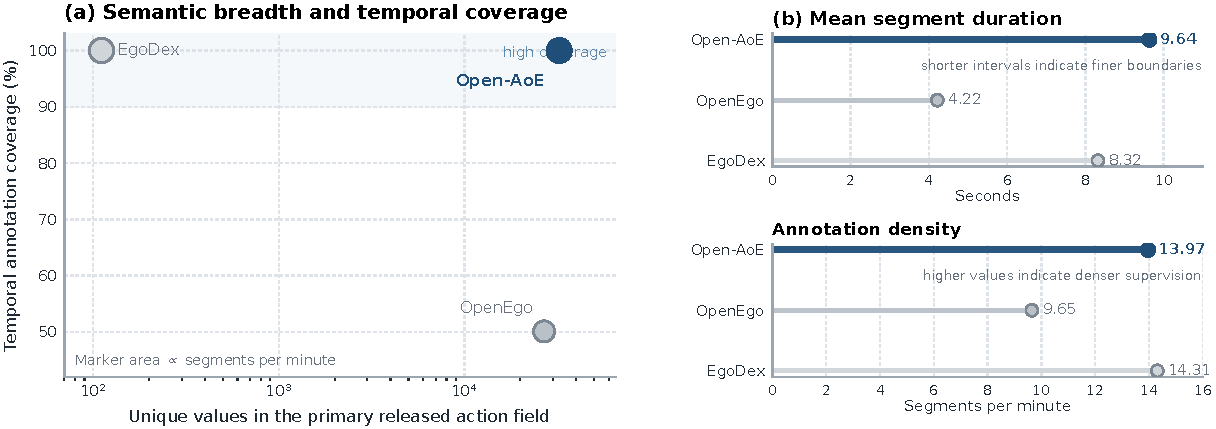
\includegraphics[width=\linewidth]{figures/fig_temporal_semantic.pdf}
    \caption{
    \textbf{Semantic breadth and temporal annotation characteristics across datasets.}
    (a) Number of unique entries in the primary released action-annotation field versus temporal annotation coverage, with marker area proportional to annotation density, measured as the number of annotated segments per minute.
    (b) Mean segment duration and annotation density for each dataset.
    Because the datasets use different native annotation schemas, vocabulary size reflects the breadth of the released semantic supervision rather than a controlled vocabulary comparison under a shared ontology.
    }
    \label{fig:temporal_semantic}
\end{figure*}

\subsection{Semantic Breadth and Temporal Completeness}

We next examine the semantic breadth and temporal structure of the released action annotations. %
Temporal coverage is defined as the fraction of the evaluated sequence timeline covered by at least one action segment, measuring the continuity of semantic supervision over the underlying video. %
The released action vocabulary is quantified by the number of unique entries in each dataset's primary action-annotation field. %
Because the datasets follow different native annotation schemas, this measure reflects the breadth of semantic supervision exposed by each release rather than a controlled comparison under a shared action ontology. %
We further characterize annotation structure using mean segment duration and annotation density, defined as the number of annotated segments per minute. %
The former captures the typical temporal extent of individual action annotations, whereas the latter reflects their frequency along the video timeline. %
Taken together, these metrics capture complementary aspects of supervision: vocabulary size reflects semantic breadth, temporal coverage measures annotation completeness, and segment duration and density characterize the granularity of localized action annotation.

As illustrated in Fig.~\ref{fig:temporal_semantic}, Open-AoE combines broad natural-language supervision with near-complete temporal coverage. %
Its primary action field comprises 32,407 distinct natural-language descriptions, compared with 26,864 native labels in OpenEgo and 111 categorical action classes in EgoDex. %
Beyond these descriptions, Open-AoE includes structured semantic fields with 8,030 object strings, 175 action verbs, and 135 scene labels, enabling each action interval to be represented at multiple levels of semantic abstraction. %
Its annotations cover 99.99\% of the evaluated timeline, substantially exceeding the 50.1\% coverage of OpenEgo, while retaining a high annotation density of 13.97 segments per minute. %
EgoDex achieves complete clip-level label coverage and a slightly higher segment density, but relies on a substantially smaller categorical action vocabulary. %
Overall, Open-AoE combines open-vocabulary semantic breadth with near-continuous temporal alignment and densely localized action supervision, without compromising annotation completeness.

\begin{figure*}[t]
    \centering
    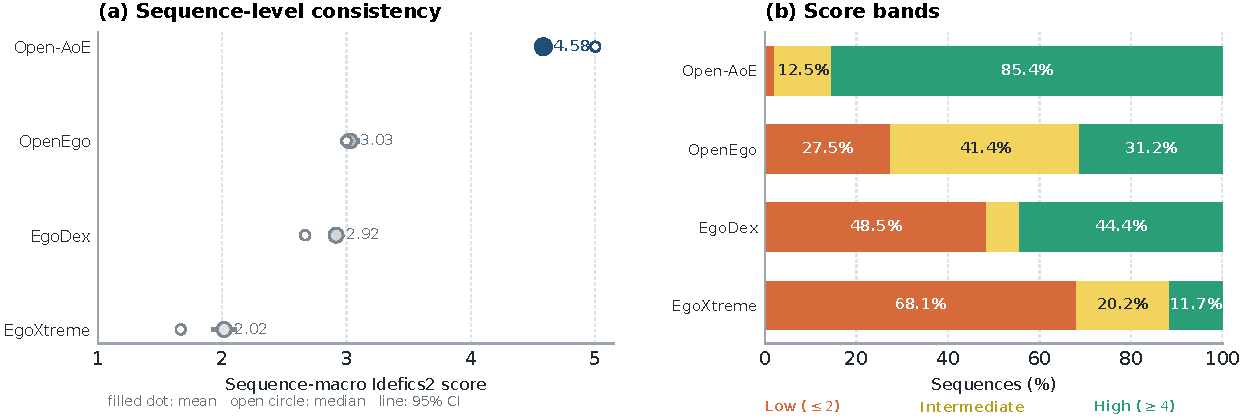
\includegraphics[width=1.0\linewidth]{figures/fig_vlm_consistency.pdf}
    \caption{
    \textbf{Sequence-level image-annotation consistency across datasets.}
    (a) Sequence-macro means, sequence-level medians, and 95\% bootstrap confidence intervals for the mean Idefics2 consistency score.
    (b) Fractions of sequences in the low ($\leq 2$), intermediate ($2<\cdot<4$), and high ($\geq 4$) score ranges.
    }
    \label{fig:vlm_consistency}
\end{figure*}

\subsection{Image-Annotation Consistency}

We assess whether the released action annotations are supported by the corresponding visual content using Idefics2~\cite{laurencon2024idefics2} as a shared vision-language evaluator. %
Let $a_{q,t}\in[1,5]$ denote the consistency score assigned to the $t$-th sampled frame of sequence $q$. %
The sequence-macro score is defined as \begin{equation} S_{\mathrm{macro}} = \frac{1}{Q} \sum_{q=1}^{Q} \left( \frac{1}{T_q} \sum_{t=1}^{T_q} a_{q,t} \right), \end{equation}
where $Q$ is the number of evaluated sequences and $T_q$ is the number of sampled frames in sequence $q$. % 
Frame-level scores are first averaged within each sequence and then across sequences, thereby assigning equal weight to each sequence and preventing longer recordings from dominating the dataset-level estimate. %
Higher scores indicate stronger agreement between the released annotations and the sampled visual evidence.

As shown in Fig.~\ref{fig:vlm_consistency}, Open-AoE achieves a sequence-macro score of $4.583/5$, substantially exceeding those of OpenEgo ($3.029$), EgoDex ($2.916$), and EgoXtreme ($2.015$). %
Its 95\% bootstrap confidence interval is $[4.557,\,4.608]$. %
This advantage is also evident in the score distribution: 85.4\% of Open-AoE sequences attain a mean consistency score of at least 4, whereas only 2.2\% score at or below 2. %
The higher aggregate score therefore reflects a broad concentration of sequences near the upper end of the scoring range rather than a small subset of exceptionally high-scoring cases. % 
Because the datasets differ in their native annotation schemas and levels of textual detail, these results should be interpreted as a cross-dataset audit of image-annotation support under a shared evaluator rather than as a fully controlled benchmark of annotation accuracy.

\begin{figure*}[t]
    \centering
    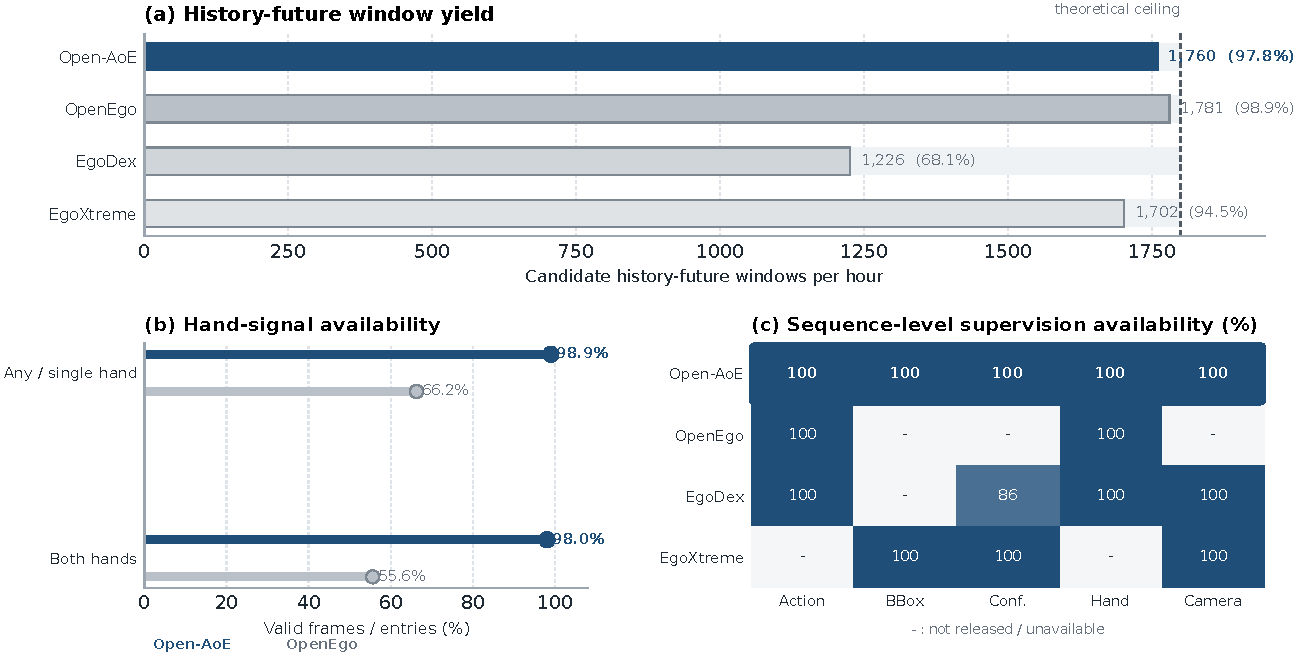
\includegraphics[width=\linewidth]{figures/fig_training_utility.pdf}
    \caption{
    \textbf{Training-sample yield and multimodal supervision availability across datasets.}
    (a) Candidate history-future windows obtained per hour using 2~s of history, 2~s of future context, and a 2~s stride, together with the retention rate relative to the no-boundary ceiling of 1,800 windows per hour.
    (b) Availability of native hand signals, distinguishing entries with at least one valid hand from those with valid signals for both hands.
    (c) Sequence-level availability of action annotations, bounding boxes, annotation confidence, hand pose, and camera pose; ``-'' indicates that the corresponding field is not released or unavailable.
    }
    \label{fig:training_utility}
\end{figure*}

\subsection{Training-Window Retention and Multimodal Completeness}

We finally assess how efficiently the released sequences can be converted into temporally aligned training samples and whether the principal supervision signals required by downstream embodied-learning pipelines are jointly available. %
For a sequence $q$ of duration $L_q$, we construct candidate samples using a history horizon of $h=2$~s, a future horizon of $f=2$~s, and a temporal stride of $\Delta=2$~s. %
The number of candidate windows is defined as
\begin{equation}
N_q
=
\max\!\left(
0,\,
\left\lfloor \frac{L_q-h-f}{\Delta} \right\rfloor + 1
\right).
\end{equation}

The history-future window yield and normalized retention are then defined as
\begin{equation}
Y_{\mathrm{window}}
=
\frac{\sum_q N_q}{\sum_q L_q/3600},
\qquad
\eta_{\mathrm{window}}
=
\frac{Y_{\mathrm{window}}}{3600/\Delta},
\end{equation}
where $\eta_{\mathrm{window}}$ measures retention relative to the no-boundary ceiling of $3600/\Delta=1{,}800$ windows per hour. %
This metric isolates losses induced by sequence boundaries and temporal discontinuities, excluding task-specific filtering imposed by individual downstream models. %
We additionally evaluate native hand-signal availability using the released validity information, distinguishing between entries with at least one valid hand and those with valid signals for both hands. %
At the sequence level, we record the availability of five principal supervision modalities: action annotations, bounding boxes, annotation confidence, hand pose, and camera pose.

As shown in Fig.~\ref{fig:training_utility}, Open-AoE yields approximately 1,760 candidate history-future windows per hour, corresponding to 97.8\% of the theoretical ceiling. %
This small gap from the no-boundary limit indicates that its temporal continuity enables dense extraction of fixed-context training samples with minimal loss at sequence boundaries. %
Open-AoE also exhibits substantially higher native hand-signal availability than OpenEgo, with 98.93\% of evaluated entries containing at least one valid hand signal and 98.02\% containing valid signals for both hands. %
Moreover, it is the only evaluated release in which all five supervision modalities are available with near-universal sequence-level coverage. %
Bounding-box quality is similarly high, with 100\% valid boxes, 98.39\% fully contained within the image boundaries, a mean confidence of 0.947, and a 10th-percentile confidence of 0.950. %
These results show that Open-AoE combines high temporal sample retention with dense, jointly available semantic, geometric, hand-motion, and camera-motion supervision, thereby reducing the modality filtering and temporal alignment required before downstream VLA, world-model, and human-to-robot training.
